\documentclass[a4paper, titlepage]{article}

% For equations
\usepackage{amsmath}

% For including figures
\usepackage{graphicx}
\usepackage{float}

% Bibiliography setup
\usepackage[square]{natbib}
\bibliographystyle{agsm}
\usepackage[nottoc]{tocbibind}

% For typesetting matlab
\usepackage{listings}
\usepackage{color} %red, green, blue, yellow, cyan, magenta, black, white
\definecolor{mygreen}{RGB}{28,172,0} % color values Red, Green, Blue
\definecolor{mylilas}{RGB}{170,55,241}

\lstset{language=Matlab,%
    basicstyle=\small,
    breaklines=true,%
    frame = single,
    morekeywords={matlab2tikz},
    keywordstyle=\color{blue},%
    morekeywords=[2]{1}, keywordstyle=[2]{\color{black}},
    identifierstyle=\color{black},%
    stringstyle=\color{mylilas},
    commentstyle=\color{mygreen},%
    showstringspaces=false,
    numbers=left,%
    numberstyle={\tiny \color{black}},% size of the numbers
    numbersep=9pt, % this defines how far the numbers are from the text
    emph=[1]{for,end,break},emphstyle=[1]\color{red}, %some words to emphasise
    %emph=[2]{word1,word2}, emphstyle=[2]{style},    
}


%\title{Assignment 3\\
%System description and analysis\\
%\large EEA004}
%\author{Dan Thilderkvist, Philip Gutierrez}

\begin{document}

%\maketitle

\begin{titlepage}
  \begin{center}
    \vspace*{1cm}
    
\includegraphics[scale=1.0]{../figures/hig_logo_eng.png}\\
    \vspace{1.5cm}
    \large EEA004 - Multivariable and Nonlinear Control Systems\\
    \large Assignment 3\\
    \vspace{1.5cm}
    Group 4\\
    Dan Thilderkvist and Philip Gutierrez\\
    dan.thilderkvist@hotmail.com philipgutierrez67@gmail.com\\
    Files: main.m\\
    
    \vspace{1cm}
    \today
  \end{center}
\end{titlepage}

\tableofcontents
\clearpage



\section{Introduction}

This assignment is a continuation of the previous two assignments where an air handler is analyzed.
Here we will look closer at two of the non-linear components of the system, namely the heater and the valve that controls it.
Both the heater and the valve have non-linear, but complementary, characteristics which compensate for each other.  However, the valve also exhibits valve authority effect which compromises the compensation between heater and valve.  These non-linearities will be analyzed closer. 
\citep[p.123]{glad00}

\subsection{Theory}

\subsubsection{Circle Criterion}
The circle criterion can be used to check input-output stability of a nonlinear system, assuming that system can be divided into two cascaded blocks $f(\cdot)$ and $G(s)$, the former encapsulating all nonlinearities of the system.
The nonlinearity $f(\cdot)$ is assumed static and the dynamic linear part $G(s)$ has no poles in the right hand half-plane.
The circle criteria is an extension of the small gain theorem that is less restrictive.
Further, assume the nonlinear function can be enclosed by the cone-shaped region bounded by two linear functions $k_1y$ and $k_2y$, see figure \ref{fig:cirEx} as an example.

\begin{equation}
k_1 \leq \frac{f(y)}{y} \leq k_2 
\end{equation} 

If two such constants $k_1$ and $k_2$ can be found for $f(\cdot)$, the circle criteria claim that the system is input-output stable if the Nyquist curve of $G(i_\omega)$ does not enter or enclose the circle that cross the real axis at $-\frac{1}{k_1}$ and $-\frac{1}{k_2}$.
It shall be noted that not full-filling the circle criteria does not directly imply instability. \citep[~p.329-334]{glad00}

\begin{figure}[h!]
\center
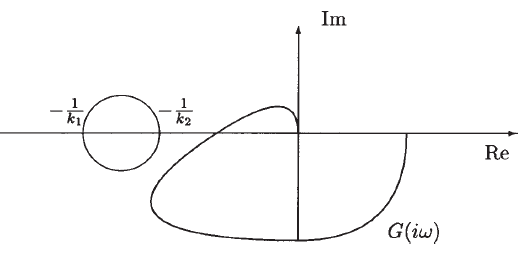
\includegraphics[scale=1]{../figures/circleExample.png}
\caption{Example of circle criteria with with the Nyquist curve $G(i\omega)$ and the circle $\left(-\frac{1}{k_1}, -\frac{1}{k_2}\right)$. This example show the criteria met as the curve does not enter the circle nor enclose it. \citep[~p.333]{glad00}}
\label{fig:cirEx}
\end{figure}



\subsubsection{Describing Function}
Assume the input of a static nonlinearity $f(.)$ is sinusoidal:

\begin{equation}
	e(t) = Csin(wt)
	\label{equ:input_e}
\end{equation}

then we would expect the output $w(t)$ to also be periodic of the form:

\begin{equation}
	w(t) = f(Csin(wt))
\end{equation}

Since this output is periodic, it may be expanded into a Fourier series such as:

\begin{equation}
	w(t) = \sum{a_{n}cos(nwt)+b_{n}sin(nwt)}
\end{equation}

where the constant term of the Fourier series can be assumed to be zero if we assume $f(.)$ is odd \citep[p. 358]{glad00}.  If we further assume that the system has a low pass characteristic, then Fourier components with angular frequencies $2w$, $3w$ and so on, can be ignored and $w(t)$ can be approximated using only the first terms of the Fourier series.  With this, $w(t)$ can be simplified as:

\begin{equation}
	w(t) = \sqrt{a_{1}^2+b_{1}^2}sin(wt+arctan(a_{1}/b_{1}))
\end{equation}

As $w(t)$ enters the system transfer function $G(.)$, the output $y(t)$ will be scaled by $|G(.)|$ and phase shifted by $arg(G(.))$, and $y(t)$ may be written as:

\begin{equation}
	y(t) = -\sqrt{a_{1}^2+b_{1}^2}|G(iw)|sin(wt+arctan(a_{1}/b_{1})+arg(G(iw)))
	\label{equ:output_y}
\end{equation}
 

We define a function, called the describing function, to be \citep[p. 358]{glad00}:

\begin{equation}
	Y_{f}(C) = \frac{b(C)+ia(C)}{C}
	\label{equ:descrbingFunction}
\end{equation}

With this definition we note that

\begin{equation}
	|Y_{f}(C)|C = \sqrt{a_{1}^2+b_{1}^2}
\end{equation}

and

\begin{equation}
	arg(Y_{f}(C)) = arctan(a/b)
\end{equation}

To reach a condition of Harmonic Balance we wish to equate (\ref{equ:output_y}) with our assumed input of (\ref{equ:input_e}).   
In particular, we need to match the amplitudes and match the phase shifts (where $\pi$ is used because of the minus sign in $y(t)$). 

\begin{equation}
\begin{split}
	|Y_{f}(C)|C|G(iw)| &= C \\
	arg(Y_{f}(C))+arg(G(iw)) &= \pi
\end{split}
\end{equation}

Under these conditions, self-sustained oscillation may occur.  The above expressions may also be written as \citep[p. 359]{glad00}:

\begin{equation}
	Y_{f}(C)G(iw) = -1
\label{equ:selfOsc}
\end{equation}
 
 
 
 
\section{Method}
The following sections describe the methods used to obtain the results presented in this report.


\subsection{System Transfer Function}
In order to control the heater system, a valve is used.
Since the heater is nonlinear, a valve with complementary nonlinearity is used and the system is now linear.
However the valve does not completely complement the system nonlinearity and hence some nonlinearity remains, called valve authority effect.
The linear part of complete system to be controlled is provided in the assignment and is specified to be:

\begin{equation}
	G(s) = \frac{1}{(s^2+s+1)(s+3)}
	\label{equ:system}
\end{equation}

The nonlinearity introduced by the valve is considered to be static.  Additionally, the valve has a gain $K_{vs}$, known as the "valve coefficient", and is available only at specific values.
With the addition of the gain $K_{vs}$, the linear part of the system become:

\begin{equation}
	G_{K_{vs}}(s) = \frac{K_{vs}}{(s^2+s+1)(s+3)}, \; K_{vs}=1, 1.6, 2.5, 4, 6.3, 10, 16.
	\label{equ:systemTF}
\end{equation}

The nonlinear part of the system $f(\cdot)$, introduced as the valve authority effect is not explicitly known.

\subsection{Circle Criteria without Valve Saturation}

The circle criteria will be used to identify the valve with maximum power that can be used.  The exact nonlinearity caused by valve authority is not known, but it is specified to be limited inside the region bounded by the blue arches as seen in figure \ref{fig:valvepower}.

\begin{figure}[h!]
\center
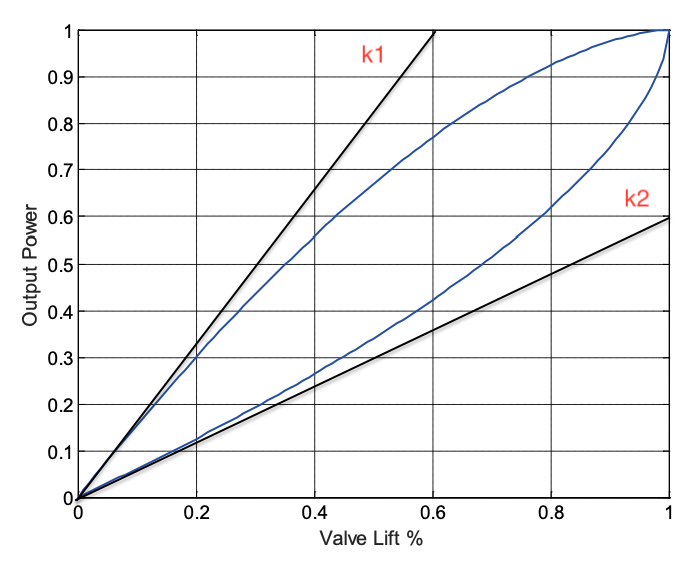
\includegraphics[scale=0.25]{../figures/valveOutputPower.png}
\caption{Valve Output Power}
\label{fig:valvepower}
\end{figure}

To apply the circle criteria, the region of known nonlinearity is bounded by two lines with slopes $k_{1}$ and $k_{2}$.  By inspection, these slopes are chosen to form a region that includes the known region of nonlinearity of the valves.  From figure \ref{fig:valvepower} we find these slopes to be:

\begin{equation}
\begin{split}
k_{1} &= \frac{1-0}{0.6-0} = 1.6 \\
k_{2} &= \frac{0.6-0}{1-0} = 0.6
\end{split}
\label{equ:k_values}
\end{equation}

The values of $k_{1}$ and $k_{2}$ are used to form an exclusion region in the Nyquist diagram bounded by a circle which intersects the real axis at $-1/k_{1}$ and $-1/k_{2}$, results figure \ref{fig:circCrit}.

With the circle criterion, input-output stability is verified if the Nyquist curve of $G_{K_{vs}}(i\omega)$ does not enter or enclose the exclusion region.

We proceed to generate a Nyquist diagram for each value of $K_{vs}$ specified in \ref{equ:systemTF}, and superimpose a circle region of exclusion in each graph, see figure \ref{fig:circCrit}.
For stability, the Nyquist curve must not enter or encircle the area of exclusion.

\subsection{Circle Criteria with Valve Saturation}

For a valve with saturation, the circle of exclusion is extended to have infinite radius by allowing $k_{2}$ to approach the x-axis and become zero.  This circle with infinite radius will appear as a vertical line in the Nyquist plots, figure \ref{fig:circCrit}.

The circle criterion can be applied as before, and stability is achieved as long as the Nyquist curve does not cross the vertical line.

\subsection{Describing Function}

An ideal relay can be modeled as \citep[p. 358]{glad00}:

\begin{equation}
\begin{split}
f(e) = \begin{cases}
1 & e > 0 \\
-1 & e <0
\end{cases}
\end{split}
\label{equ:relay}
\end{equation}

By using (\ref{equ:descrbingFunction}) the resulting describing function of the relay can be found to be \citep[P. 359]{glad00}:

\begin{equation}
Y_{f}(C) = \frac{4}{\pi C}
\label{equ:relayDescribingFuntion}
\end{equation}

For oscillation to occur, the relationship (\ref{equ:selfOsc}) must be satisfied.  Since the describing function of the relay (\ref{equ:relayDescribingFuntion}) is real and positive, we observe that $G(iw)$ in (\ref{equ:selfOsc}) must be real and negative.

To accomplish this, the system transfer function (\ref{equ:systemTF}) yields:

\begin{equation}
\begin{split}
G(iw) &= \frac{K_{vs}}{((iw)^2+(iw)+1)((iw)+3)}\\
&= \frac{K_{vs}[(3-4w^2)-i(4w-w^3)]}{[(3-4w^2)+i(4w-w^3)][(3-4w^2)-i(4w-w^3)]}
\end{split}
\label{equ:systemTFiw}
\end{equation}

This equation is real when:

\begin{equation}
4-w^2 = 0 => w=2
\label{equ:systemTFreal}
\end{equation}

At this frequency we find that equation (\ref{equ:systemTFiw}) provides:

\begin{equation}
G(i2) = \frac{-K}{13}
\label{equ:systemTFw2}
\end{equation}

which indeed is real and negative as required.

Finally, with the describing function of the relay specified in  (\ref{equ:relayDescribingFuntion}) and $G(iw)$ evaluated at the oscillating frequency $w=2$ provided in (\ref{equ:systemTFw2}) we can use the relationship from (\ref{equ:selfOsc}) to obtain:

\begin{equation}
Y_{f}(C)G(iw) = \frac{4}{\pi C}\frac{(-K)}{13} = -1
\label{equ:selfOscw2}
\end{equation}

The assignment asks for a magnitude of oscillation below $C < 0.5$.
Therefore, from (\ref{equ:selfOscw2}) above we find the maximum value of $K_{vs}$ to be:

\begin{equation}
K_{MAX} = \frac{13C_{MAX}\pi}{4} < \frac{13 \cdot 0.5\pi}{4}= 5.10
\label{equ:maximum_k}
\end{equation}

\subsection{Graphical Solution using Describing Function}

As an alternative, equation (\ref{equ:selfOsc}) can be solved graphically by finding the intersection of the two graphs:

\begin{equation}
G(iw) = \frac{-1}{Y_{f}(C)} = -\frac{C\pi}{4}
\end{equation}

where the graph of $G(iw)$ is simply the Nyquist diagram of $G(iw)$ with the plot of $-1/Y_{f}(C)$ superimposed.

The plot of $-1/Y_{f}(C)$ with varying values of C is included in the Nyquist diagram in figure \ref{fig:circCrit}, and the point where $C=0.5$ is marked with a red circle.

Note also that $-1/Y_{f}(C)$ goes from right to left in the diagram with increasing C, so the intersection of the two graphs must occur to the right of the circle to have $C < 0.5$ as required.

Parenthetically, note that $-1/Y_{f}(C)$ is negative and real, so it will simply appear as a straight line on the negative real axis. 


\section{Results}

\subsection{Circle Criteria Results}
Figure \ref{fig:circCrit} show the Nyquist curves of $G_{K_{vs}}(i\omega)$ and include a circle of exclusion which is bounded by $-1/k_{1}$ and $-1/k_{2}$.  The diagram also include an exclusion region bounded by $-1/k_{1}$ (shown as a vertical line in the figure) which is used when analyzing the case with saturation in the valve.

\begin{figure}[H]
\center
\includegraphics[scale=0.75]{../code/figures/circFig.png}
\caption{Nyquist diagram for $G_{K_{vs}}(i\omega)$ for applying the circle criterion. Exclusion regions are marked with thick red.}
\label{fig:circCrit}
\end{figure}

%\begin{figure}[h!]
%\center
%\includegraphics[scale=0.25]{../code/figures/nyquist1.png}
%\caption{Nyquist diagram for $K_{vs}=1.0$}
%\label{fig:nyquist1}
%\end{figure}
%
%\begin{figure}[h!]
%\center
%\includegraphics[scale=0.25]{../code/figures/nyquist2.png}
%\caption{Nyquist diagram for $K_{vs}=1.6$}
%\label{fig:nyquist2}
%\end{figure}
%
%\begin{figure}[h!]
%\center
%\includegraphics[scale=0.25]{../code/figures/nyquist3.png}
%\caption{Nyquist diagram for $K_{vs}=2.5$}
%\label{fig:nyquist3}
%\end{figure}
%
%\begin{figure}[h!]
%\center
%\includegraphics[scale=0.25]{../code/figures/nyquist4.png}
%\caption{Nyquist diagram for $K_{vs}=4.0$}
%\label{fig:nyquist4}
%\end{figure}
%
%\begin{figure}[h!]
%\center
%\includegraphics[scale=0.25]{../code/figures/nyquist5.png}
%\caption{Nyquist diagram for $K_{vs}=6.3$}
%\label{fig:nyquist5}
%\end{figure}
%
%\begin{figure}[h!]
%\center
%\includegraphics[scale=0.25]{../code/figures/nyquist6.png}
%\caption{Nyquist diagram for $K_{vs}=10$}
%\label{fig:nyquist6}
%\end{figure}
%
%\begin{figure}[h!]
%\center
%\includegraphics[scale=0.25]{../code/figures/nyquist7.png}
%\caption{Nyquist diagram for $K_{vs}=16$}
%\label{fig:nyquist7}
%\end{figure}

Figure \ref{fig:circCrit} show that the Nyquist curve crosses the circle of exclusion for $K_{vs}=6.3$.  Therefore, the maximum size valve (without saturation) is:

\begin{equation}
K_{vs} = 4.0
\label{equ:k_max_wo_saturation}
\end{equation}

Similarly, the Nyquist curve crosses the exclusion line for $K_{vs}=4.0$, showing the maximum size valve with saturation to be:

\begin{equation}
K_{vs} = 2.5
\label{equ:k_max_w_saturation}
\end{equation}

\subsection{Describing Function Results}

From the relationship given in (\ref{equ:selfOsc}) and the frequency of oscillation provided by (\ref{equ:systemTFiw}) and (\ref{equ:systemTFreal}), we find the frequency of oscillation to be:

\begin{equation}
w=2
\label{equ:omega_zero}
\end{equation}

At this frequency, equation (\ref{equ:maximum_k}) provides a maximum value of $K$ value of:

\begin{equation}
K_{MAX} < 5.10
\label{equ:k_valid}
\end{equation}

Since the valves come in specific sizes (1, 1.6, 2.5, 4.0, 6.3, 10, and 16) we find that the maximum valve coefficient is:

\begin{equation}
K_{vs} = 4.0
\label{equ:k_max}
\end{equation}

As confirmation of these results, we can inspect figure \ref{fig:circCrit} visually and note that the Nyquist curve for $K_{vs}=4.0$ crosses the real axis to the right of the red circle which indicates C=0.5.  Furthermore, $K_{vs}=6.3$ crosses the real axis to the left.  Hence, the answer in (\ref{equ:k_max}) is indeed correct. 

\section{Discussion}

For certain nonlinearities, $f(.)$, which are static and unique, we may employ the circle criterion to determine stability if the following conditions are met:

\begin{equation}
\begin{split}
f(0) &= 0 \\
k_{1} {\leq} \frac{f(y)}{y} &{\leq} k_{2}, \; y {\neq} 0
\end{split}
\end{equation}

Illustrated in figure \ref{fig:valvepower}, $k_{1}$ and $k_{2}$ are chosen to fully enclose the region of known nonlinearity.  As stated earlier, a sufficient condition for input output stability is that the Nyquist curve does not enter or enclose the circle as seen in figure \ref{fig:circCrit}. It is interesting to note, however, that if the circle criterion is not satisfied, then that does not imply instability.   

Satisfying the circle criterion limits the selection of valves to the valves with smaller valve coefficients (and less valve authority).  Specifically, to those less than $K_{vs}=4.0$.

In the case of valves with saturation, further restriction is imposed and the largest valve is $K_{vs}=2.5$

Since, in general, a higher valve authority is preferred, the radius of the circle is important as an overly large radius, caused by selecting $k_{1}$ and $k_{2}$ too conservatively,  may exclude valves unnecessarily. This leads to an interesting question of absolute stability and robustness.  In other words, how close to the circle is "safe"?

Another observation from figure \ref{fig:valvepower} is that a large region of nonlinearity will require a large sector to be blocked out.  This may be a costly proposition to ensure global absolute stability, and perhaps it is possible to study absolute stability within a finite region as a compromise.

A describing function of a relay was used to analyze undesired oscillations in the system.  The task was to identify the largest valve that would limit the amplitude of oscillation to less than 0.5.
Two approaches were taken for this assignment.  First an algebraic method was used followed by a graphical approach.

An algebraic approach was possible since the system in (\ref{equ:systemTF}) and the describing function (\ref{equ:relayDescribingFuntion}) are not too complex.  However, it became evident that an algebraic approach would be limited to only relatively simple systems due to the complexity of the calculations.

The graphical solution provides a simple means to solve the describing function approach by plotting the inverse of the describing function in the Nyquist diagram and noting where the two curves intersect each other. By identifying the point on the describing function curve where $C=0.5$, it was a straight forward effort to find the largest allowable valve by noting which Nyquist curve that intersected the describing curve to the left of the $C=0.5$ point.

In both the algebraic and graphical approach, the maximum valve size was found to be $K_{vs}=4.0$.

An interesting benefit of the algebraic approach was that a maximum value of $K_{vs}=5.10$ could be obtained explicitly. This information is not evident by looking at the graphical solution alone.  The graphical solution could only help identify which of the standard valve sizes that should be chosen.    

 
\section{Conclusion}

The circle criterion is a powerful method for absolute stability analysis.  In this assignment we used the circle criterion to select a valve size that would provide maximum power given the nonlinear behavior of the valve authority effect.  The method of circle criterion was easily extended to support analysis of valves with and without saturation.

Furthermore, the method of describing function was used to analyze the harmonic balance of the system, and to choose a valve that would limit the magnitude of oscillations.  Both an algebraic and graphical approach was used, and the benefits of both approaches were discussed.

This assignment highlighted several interesting areas for future study, such as, the relationship between absolute stability and robustness, and global stability vs. stability in a finite region, and finally, generalized sector selection of the nonlinearity to reduce conservatism.   



\clearpage
\bibliography{reference}

\clearpage
\appendix

\section{Appendix}
Here is the Matlab code used to generate the results in the report and the figures.

\lstinputlisting{../code/main.m}

\end{document}